\section{Implementing the framework as an extension of the RTOS \label{sec:extension}}

For this second approach, the idea comes from our discussion with the community.
Instead of building the framework inside the kernel, we would implement the framework as a RTOS extension.
The extension would provide calls that would be used in the user-space in the application.

\subsection{Definition of RTOS extension}

Many RTOS allow developers to create their own extensions that will be used by other developers to enhance and add functionnalities to their applications.
In these extensions, we can found libraries that allow the use of FTP or COAP or even a Shell.
To use those extensions, the developer need to specify them in the \texttt{Makefile}.
Those libraries are called 'apps' for Contiki and 'modules' for RIOT OS.

\begin{minipage}{.45\textwidth}
\begin{lstlisting}[style=CStyle, language=make, caption=Example of Makefile using the app \texttt{shell} with Contiki]
CONTIKI_PROJECT = example
all: $(CONTIKI_PROJECT)
CONTIKI = ../contiki

# Using the shell app
APPS += shell 

include $(CONTIKI)/Makefile.include
\end{lstlisting}
\end{minipage}\hfill
\begin{minipage}{.45\textwidth}
\begin{lstlisting}[style=CStyle, language=make, caption=Example of Makefile using the module \texttt{shell} with RIOT OS]
APPLICATION = example
BOARD ?= native
RIOTBASE ?= $(CURDIR)/../riot

# Using the shell module
USEMODULE += shell 

include $(RIOTBASE)/Makefile.include
\end{lstlisting}
\end{minipage}

\subsection{Framework usage} % TODO - Find a better name

Let's start by explaining how the framework works with this second approach.
The idea is to be able to measure the context switching time without impacting the application.
With this in mind, we will make sure that our framework is called only two times per task iteration.
From these calls, we can deduce the context switching time.
The figure \ref{fig:internal-framework-ping} shows an example with two tasks.
The first task starts at the step A and ends at the step A'.
A context switch occurs between the step A' and the step B, this latter being the start of the second task.
The step B' is the end of the second task.
The idea is to call the framework at each step, A, A', B and B'.
The context switching time is measured between the step A' and B.
The next sections describe the implementation of this framework and what happens when it is used with our simple application.

\begin{figure}[!ht]
  \centering
  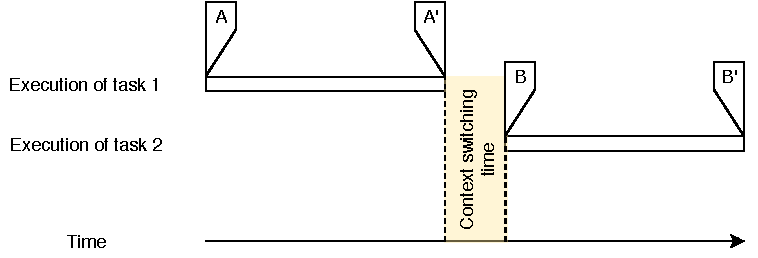
\includegraphics[scale=1]{assets/internal-framework-ping.pdf}
  \caption{\label{fig:internal-framework-ping}Pings to the framework}
\end{figure}

\subsection{Using the framework with our simple application}

To understand the implementation of the framework, we need to understand what happens when our simple application boots and then explain its implementation in the next section.

In the startup of our application, the first task is launched.
It will call the method \texttt{bench\_ping(TASK\_1)} where \texttt{TASK\_1} is the ID of the first task.
At this point, we enter in the framework-space like shown in the figure \ref{fig:extension-activity-framework}.
The framework will check if the received ID from the \texttt{bench\_ping()} call is already stored in its context.
If the received ID match the one stored in the context or if no ID is stored in the context, no context switch occcured and the framework reset its internal timer.
It also store the received ID in its context.
The stored ID is now \texttt{TASK\_1}.
Once the first task ends its iteration and will let the other task runs, it call the same method \texttt{bench\_ping(TASK\_1)} with its ID.
Once again, the framework checks the received ID and no change is detected.
It resets its internal timer.
The stored ID is still \texttt{TASK\_1}.

Now, the second task starts and call the framework with \texttt{bench\_ping(TASK\_2)} where \texttt{TASK\_2} is the ID of the second task.
The framework will detect an ID change by comparing the received ID, \texttt{TASK\_2}, with the stored ID in its context, \texttt{TASK\_1}.
This change means that a context switch occured.
We are between the step A' and B in the figure \ref{fig:internal-framework-ping}.
The framework will measure the context switching time by computing the difference between the actual timer and its internal timer.
The measure is then written on the serial port to be read by an external source like a computer.
The framework resets once again its timer and store the \texttt{TASK\_2} ID in its context.
In this way, we have computed the context switching time between the first and the second task.

\begin{figure}[!ht]
  \centering
  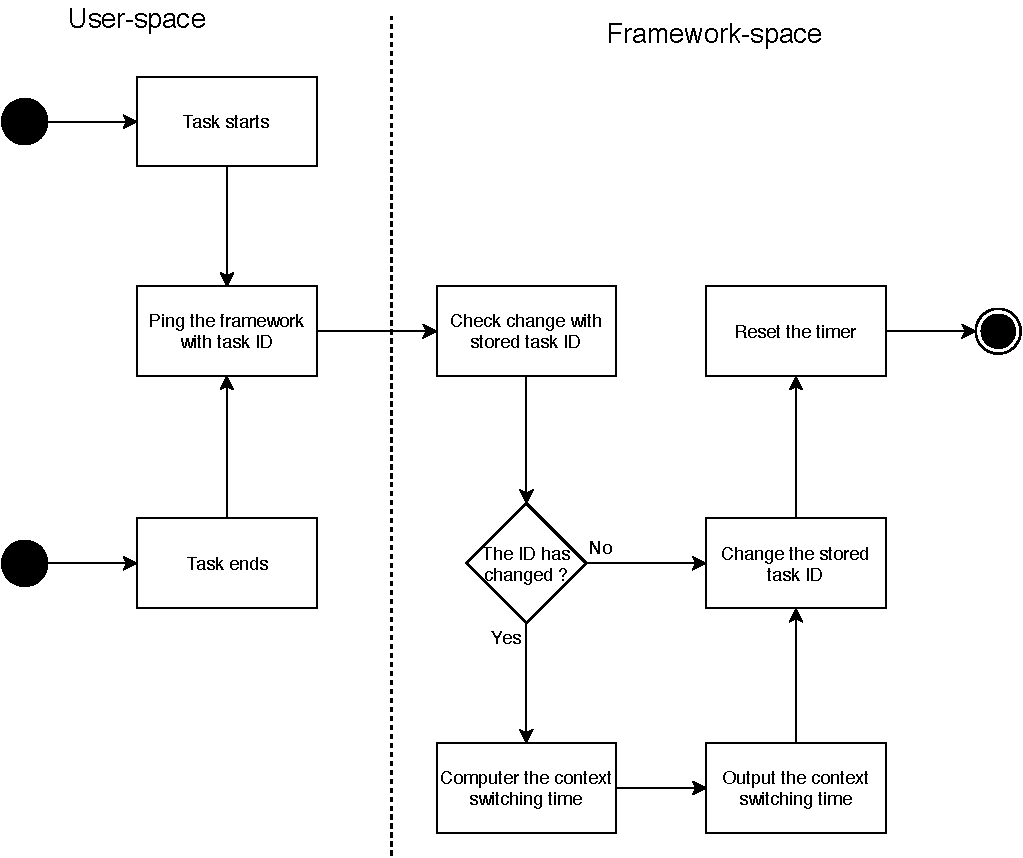
\includegraphics[scale=0.7]{assets/extension-activity-framework.pdf}
  \caption{Activity flow of the framework\label{fig:extension-activity-framework}}
\end{figure}

\subsection{Framework implementation}

\subsubsection{Task source code}
For our simple application source code, we just had to add the call \texttt{bench\_ping()} at the start and the end of each task.
The listing \ref{lst:bench-task-code} shows how, in Contiki, the task source code have changed.

\begin{lstlisting}[float, style=CStyle, label={lst:bench-task-code}, caption={Source code of the task with \texttt{bench\_ping()} calls}]
PROCESS_THREAD(task, ev, data)
{
    PROCESS_BEGIN();

    while (1)
    {
      bench_ping(TASK_ID); // Ping the framework
      // Wait for 1ms
      clock_delay_usec(1000);
      bench_ping(TASK_ID); // Ping the framework
      PROCESS_PAUSE();
    }

    PROCESS_END();
}
\end{lstlisting}

\subsubsection{Framework source code}

For the framework context, we store the received ID in the \texttt{new\_id} variable and then use the \texttt{previous\_id} variable to check if a context switch occured.
The \texttt{current\_time} variable is the interval timer.
The code of the framework context is shown in the listing \ref{lst:context-code}.

\begin{lstlisting}[style=CStyle, float, label={lst:context-code}, caption={Framework context implementation}]
struct BContext {
  uint32_t previous_id;
  uint32_t new_id;
  clock_time_t current_time;
} bench_context;
\end{lstlisting}

The \texttt{bench\_ping()} method will just saved the received ID in the \texttt{new\_id} variable and then check if a change is detected like shown in the listing \ref{lst:bench-ping-code}.

\begin{lstlisting}[style=CStyle, float, label={lst:bench-ping-code}, caption={\texttt{bench\_ping()} implementation}]
void bench_ping(uint32_t id)
{
  bench_context.new_id = id;
  if (!check_change())
  {
    bench_context.current_time = RTIMER_NOW();
  }
}
\end{lstlisting}

When a change is detected, the framework will compute the context switching time by retrieving the current time and computing its difference with \texttt{current\_time} variable.
The time is computed in ticks with the \texttt{RTIMER\_NOW()} method for a better precision.
The internal timer is then reset just before writting the measure into the serial port.
Then the measure is outputted into the serial port using the \texttt{printf()} call.
The code of this measurement is shown in the listing \ref{lst:measurement-code}.

\begin{lstlisting}[style=CStyle, float, label={lst:measurement-code}, caption={Source code of the benchmarking framework implemented in Contiki}]
// Compute the difference
clock_time_t previous = bench_context.current_time;
clock_time_t current = RTIMER_NOW();
clock_time_t result = current - previous;

// Keep the previous id for log
uint32_t previous_id = bench_context.previous_id;
// Change previous_id to new_id
bench_context.previous_id = bench_context.new_id;

bench_context.current_time = RTIMER_NOW(); // Ticks

printf("[BENCH_CONTEXT_SWITCHING] %lu %lu %lu\n", previous_id, bench_context.new_id, result);
\end{lstlisting}



% For this second approach, we decided to develop our framework as a Contiki app.
% The idea is to cause each task to ping the framework with its thread ID at the start and at the end of its execution.
% In this way, the framework will keep track of which task is running and can detect a context switch and compute its duration.

% In the figure \ref{fig:internal-framework-ping}, we can see an example of usage with two tasks.
% The task 1 pings the framework at steps A and A' with its thread ID of 1, respectively the start and the end of its execution.
% The task 2 do the same at steps B and B' but with its thread ID of 2.
% The context switch occurs between the steps A' and B and the framework can use the received pings to deduce the context switching time.

% \subsubsection{Framework implementation}
% The implementation uses an internal structure \texttt{bench\_context} to store the last thread ID received with a ping and a timer to mesure the potential context switch.
% Once a ping is received with the \texttt{bench\_ping(uint32\_t)} call, the framework store the new thread ID in its context and check if a change of thread IDs occurs with the \texttt{check\_change()} function.
% If the two thread IDs match, no context switch happened and the same task is running on the foreground.
% If the old thread ID does not match the new thread ID, it means a context switch just occur.
% The context switching time is then computed using the timer stored in the context of the framework.
% Finally, the time is reset.

% The documented source code can be found in the listing \ref{lst:internal-bench-code}.